\chapter*{Implementace}

\par V rámci této úlohy bylo ve frameworku QT vytvořené uživatelské prostředí pro tvorbu digitálního modelu terénu s využitím zmíněných algoritmů v předcházející kapitole.

\section*{Vstupní data}
\par Aplikace (obr. 5) je přizpůsobená na načítání geografických vstupních dat v Křovákově souřadnicovém referenčním systému (\verb|EPSG:5514|) ve formátu \verb|CSV|. Aplikace umí rozpoznat načítání prázdného, či nevalidního \verb|CSV| souboru. Uživatel je na takovou skutečnost upozorněn. K aplikaci jsou přiloženy testovací data ve formátu \verb|CSV| ve složce \emph{input\textunderscore files} pod názvem \verb|terrain.csv|.
\begin{figure}[H]
\centering
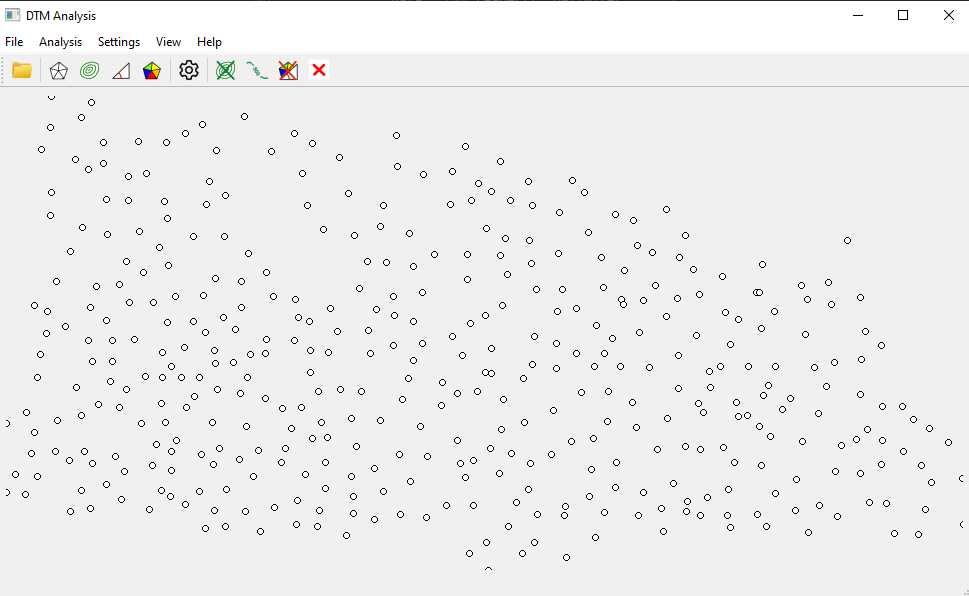
\includegraphics[width=14cm]{data_load.png}
    \caption{Ukázka načtení bodového mračna (vlastní zpracování).}
\end{figure}
\section*{Aplikace}
\par Grafické rozhraní aplikace bylo vytvořeno v prostředí \verb|Qt Creator 9.0.1| a dále upravováno v prostředí programovacího jazyka \verb|Python 3.11|. Ovladatelnost a možnosti aplikace popisuje obr. 6.

\begin{figure}[H]
\centering
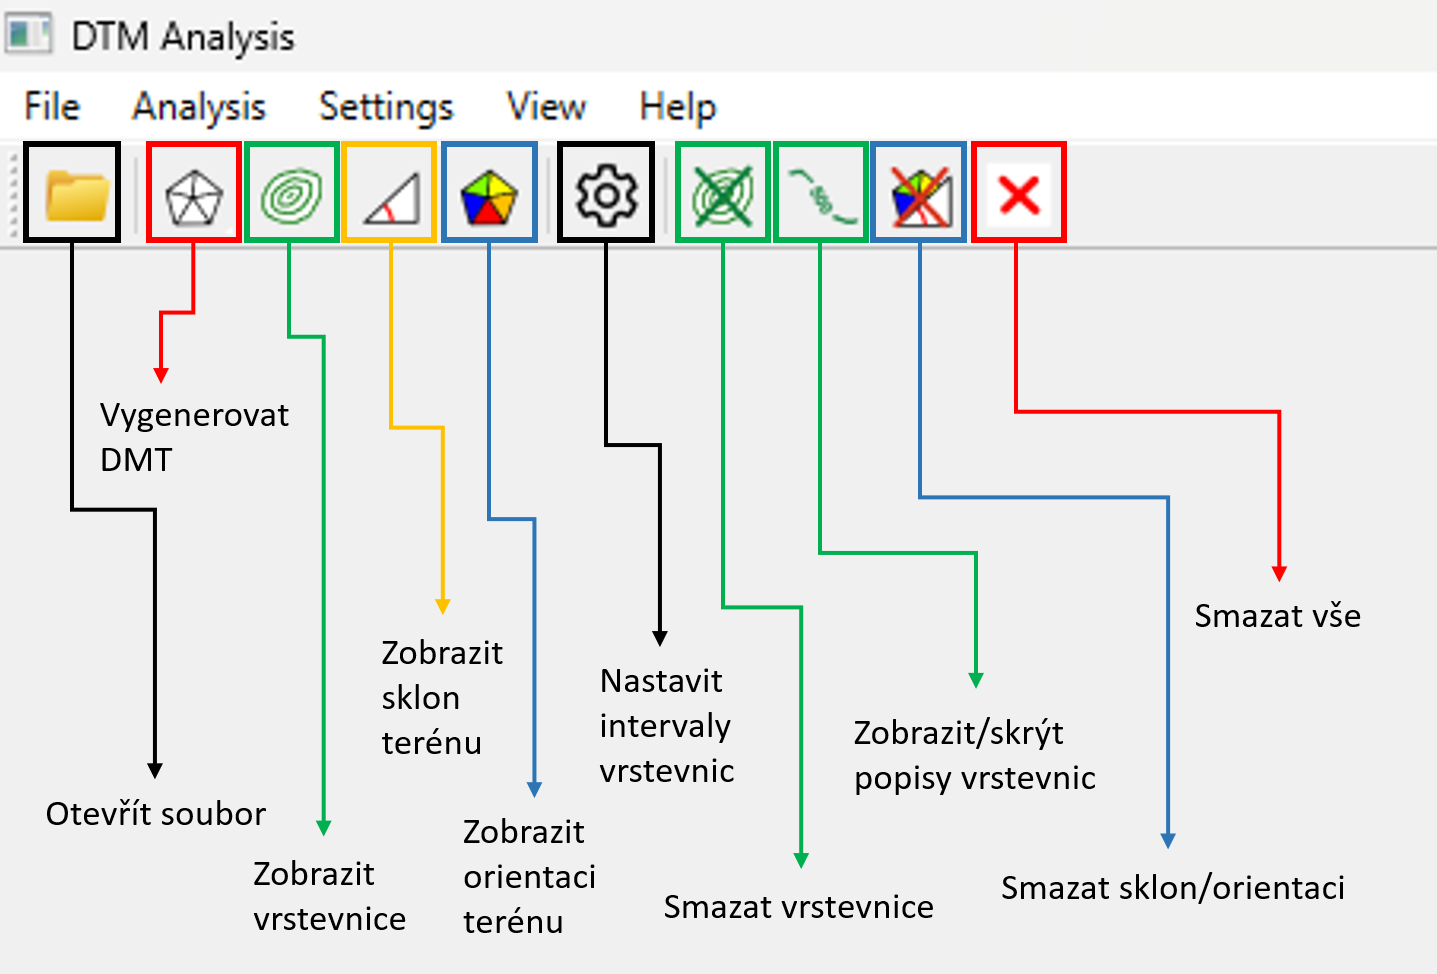
\includegraphics[width=14cm]{images/showcase.png}
    \caption{Ukázka grafického okna aplikace s popisem funkcí (vlastní zpracování).}
\end{figure}

\par Uživatel má možnost na vstupních datech provést Delaunayho triangulaci (obr. 7a). Následně lze nad vytvořenou triangulací vygenerovat vrstevnice (obr. 7b). Pro výslednou DT lze zobrazit sklon (obr. 7c) v šedotónových barvách a orientaci terénu (obr. 7d) v barevné paletě podle ESRI (Buckley 2008). Pokud uživatel spustí výpočet DT, aniž by měl načtena data, bude na tuto skutečnost upozorněn vyskakovacím oknem. Podobným způsobem se uživateli zobrazí upozornění, když klikne na výpočet vrstevnic, nebo zobrazení sklonu/orientace terénu.

\begin{figure}[H]

\begin{subfigure}{.475\linewidth}
  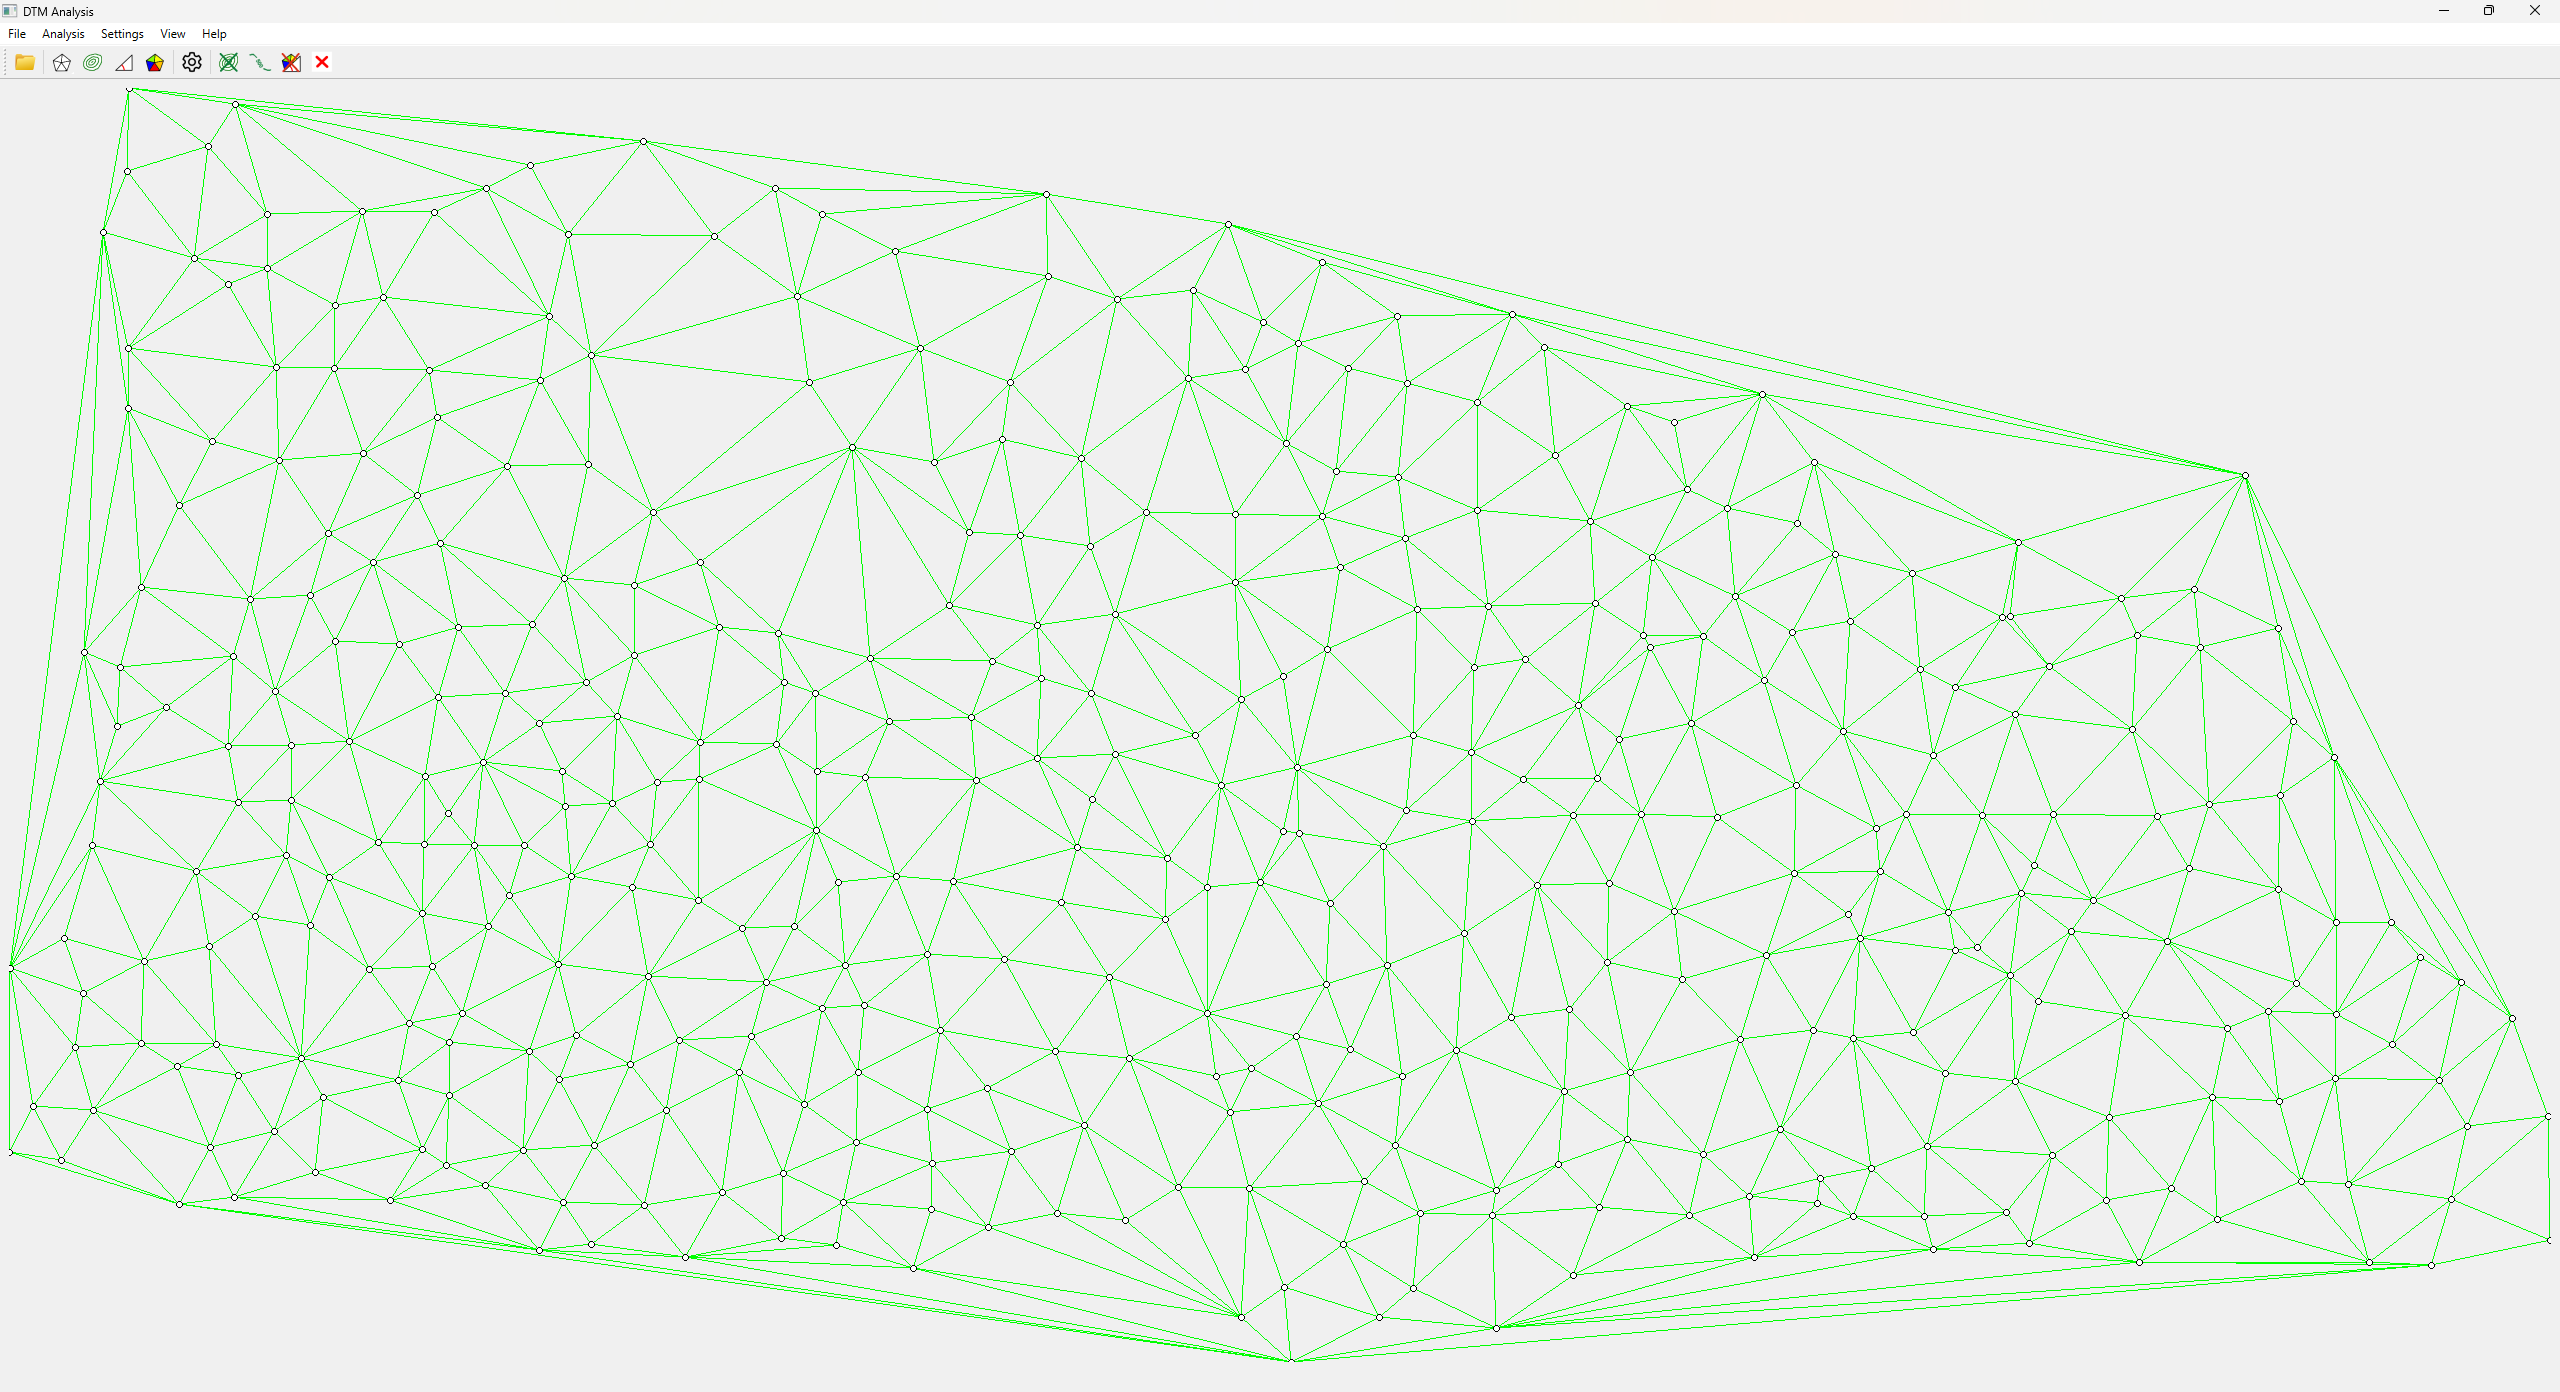
\includegraphics[width=\linewidth]{images/dtshowcase.png}
  \caption{DT nad vstupnými daty}
  \label{MLEDdet}
\end{subfigure}\hfill % <-- "\hfill"
\begin{subfigure}{.475\linewidth}
  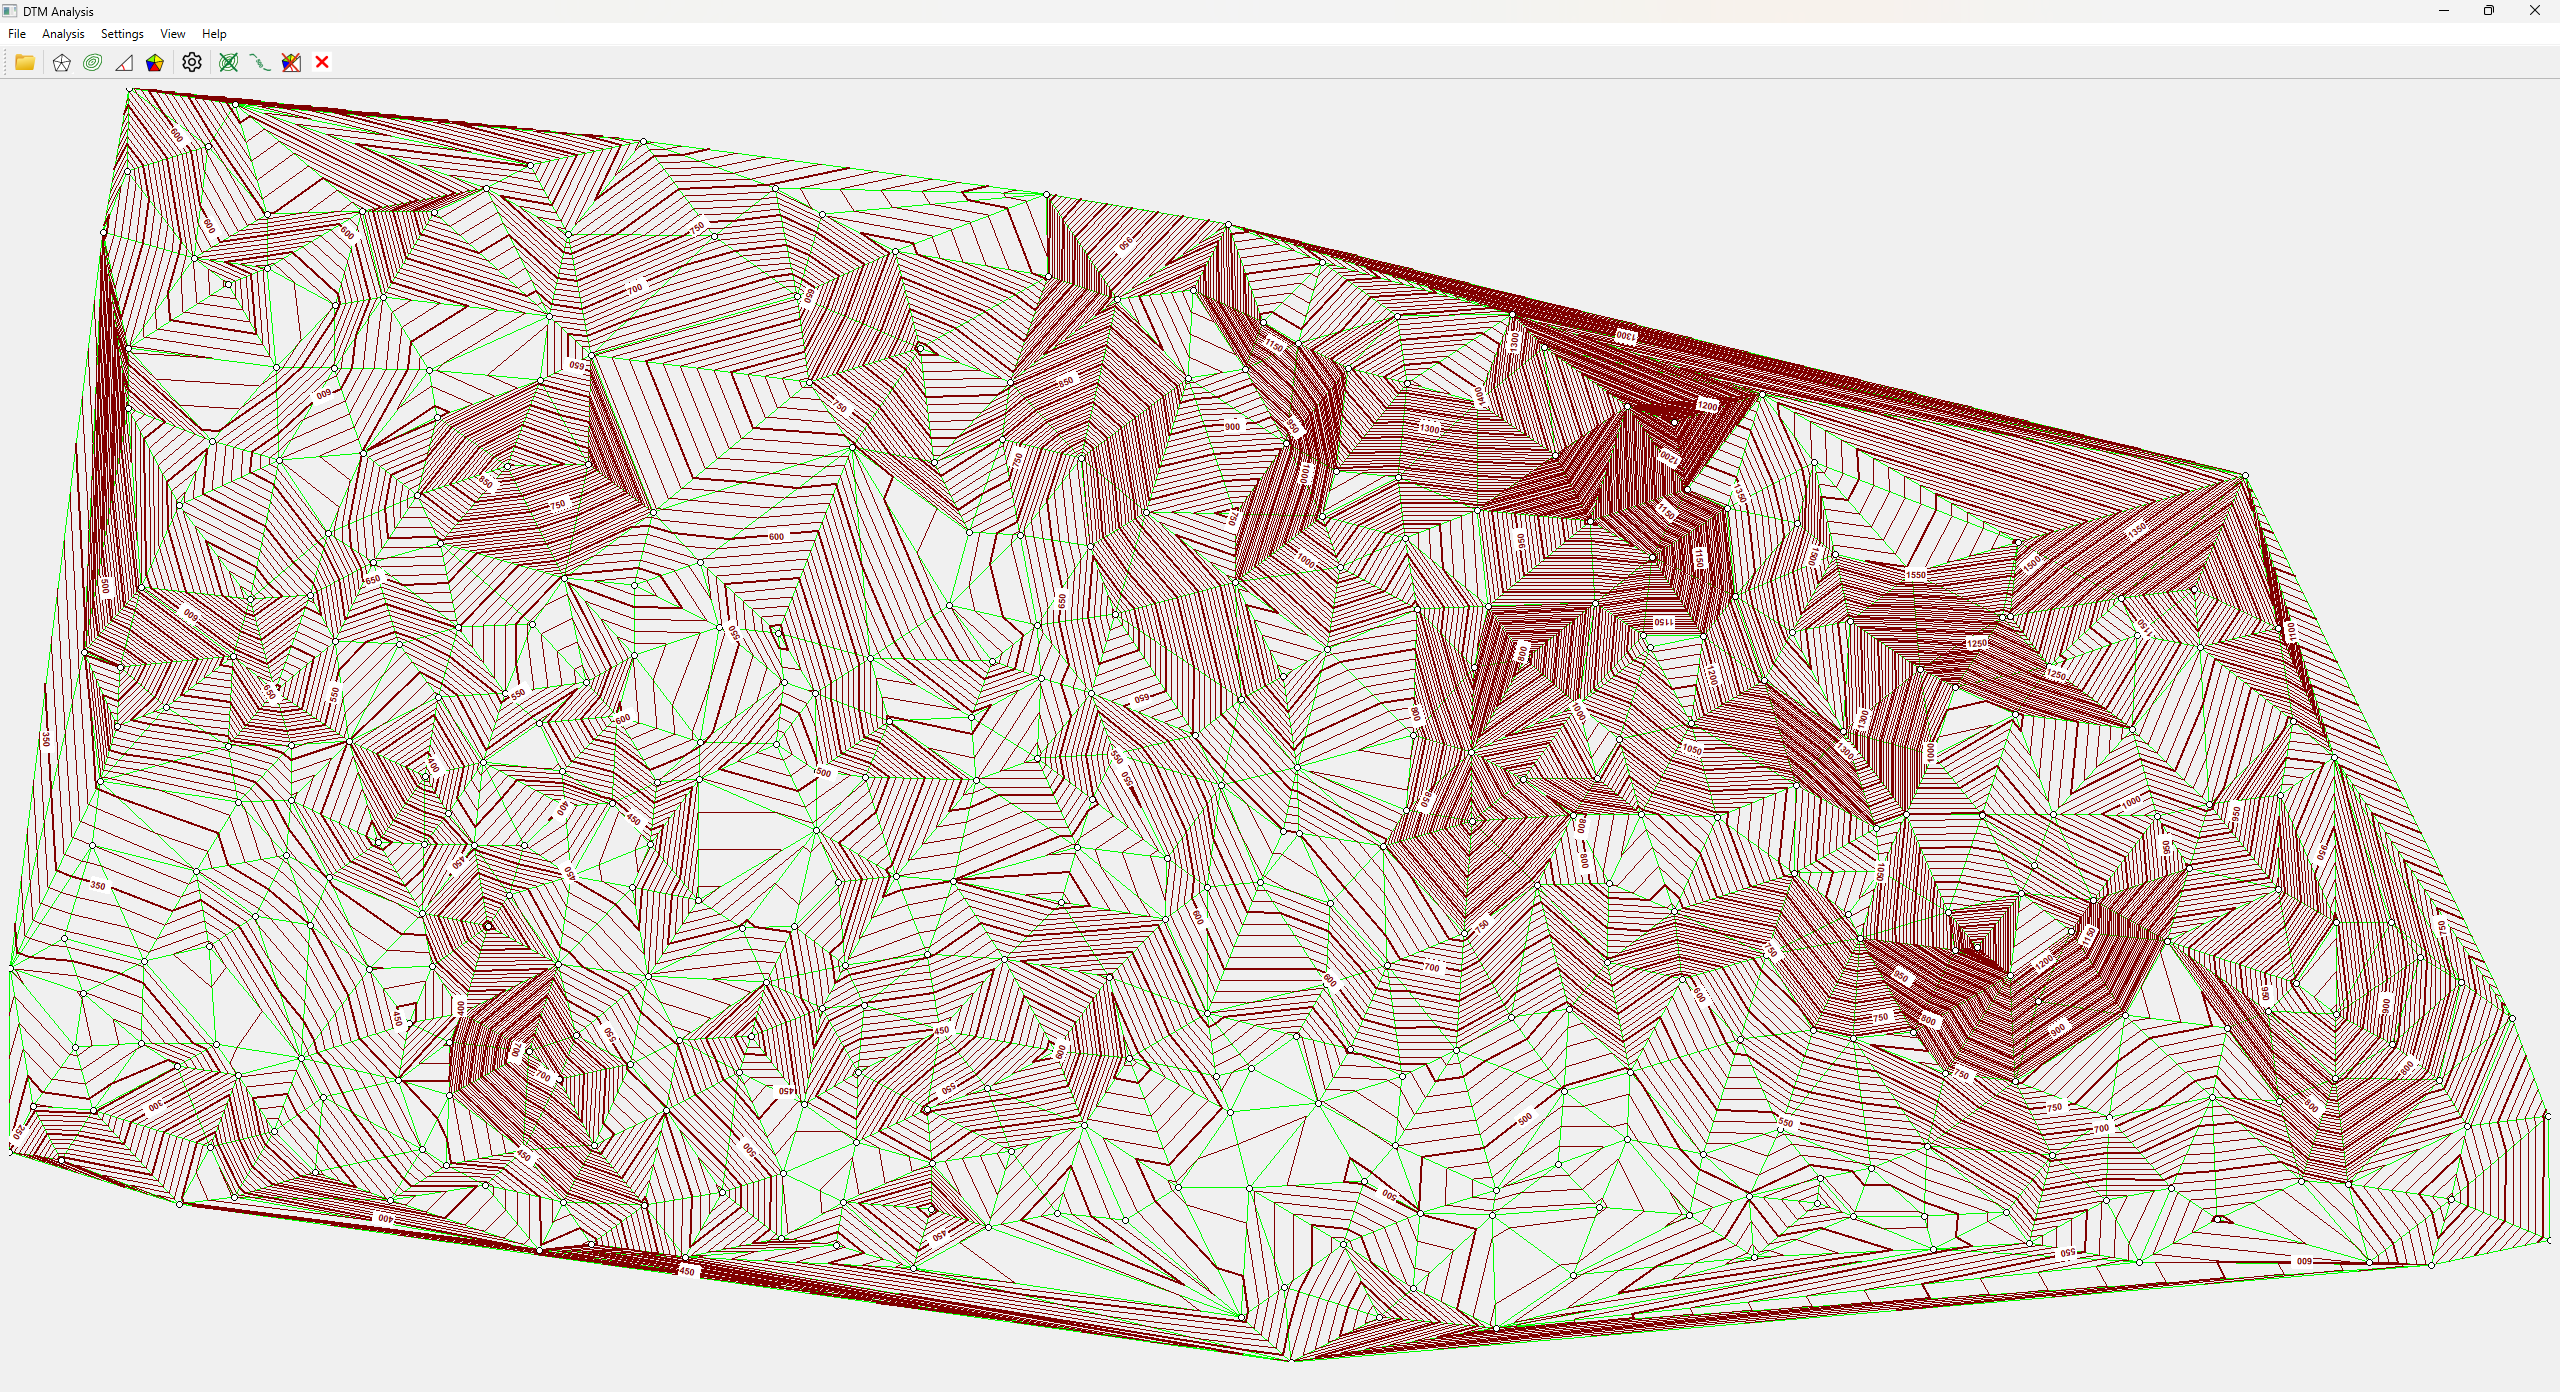
\includegraphics[width=\linewidth]{images/contourshowcase.png}
  \caption{vrstevnice}
  \label{energydetPSK}
\end{subfigure}

\medskip % create some *vertical* separation between the graphs
\begin{subfigure}{.475\linewidth}
  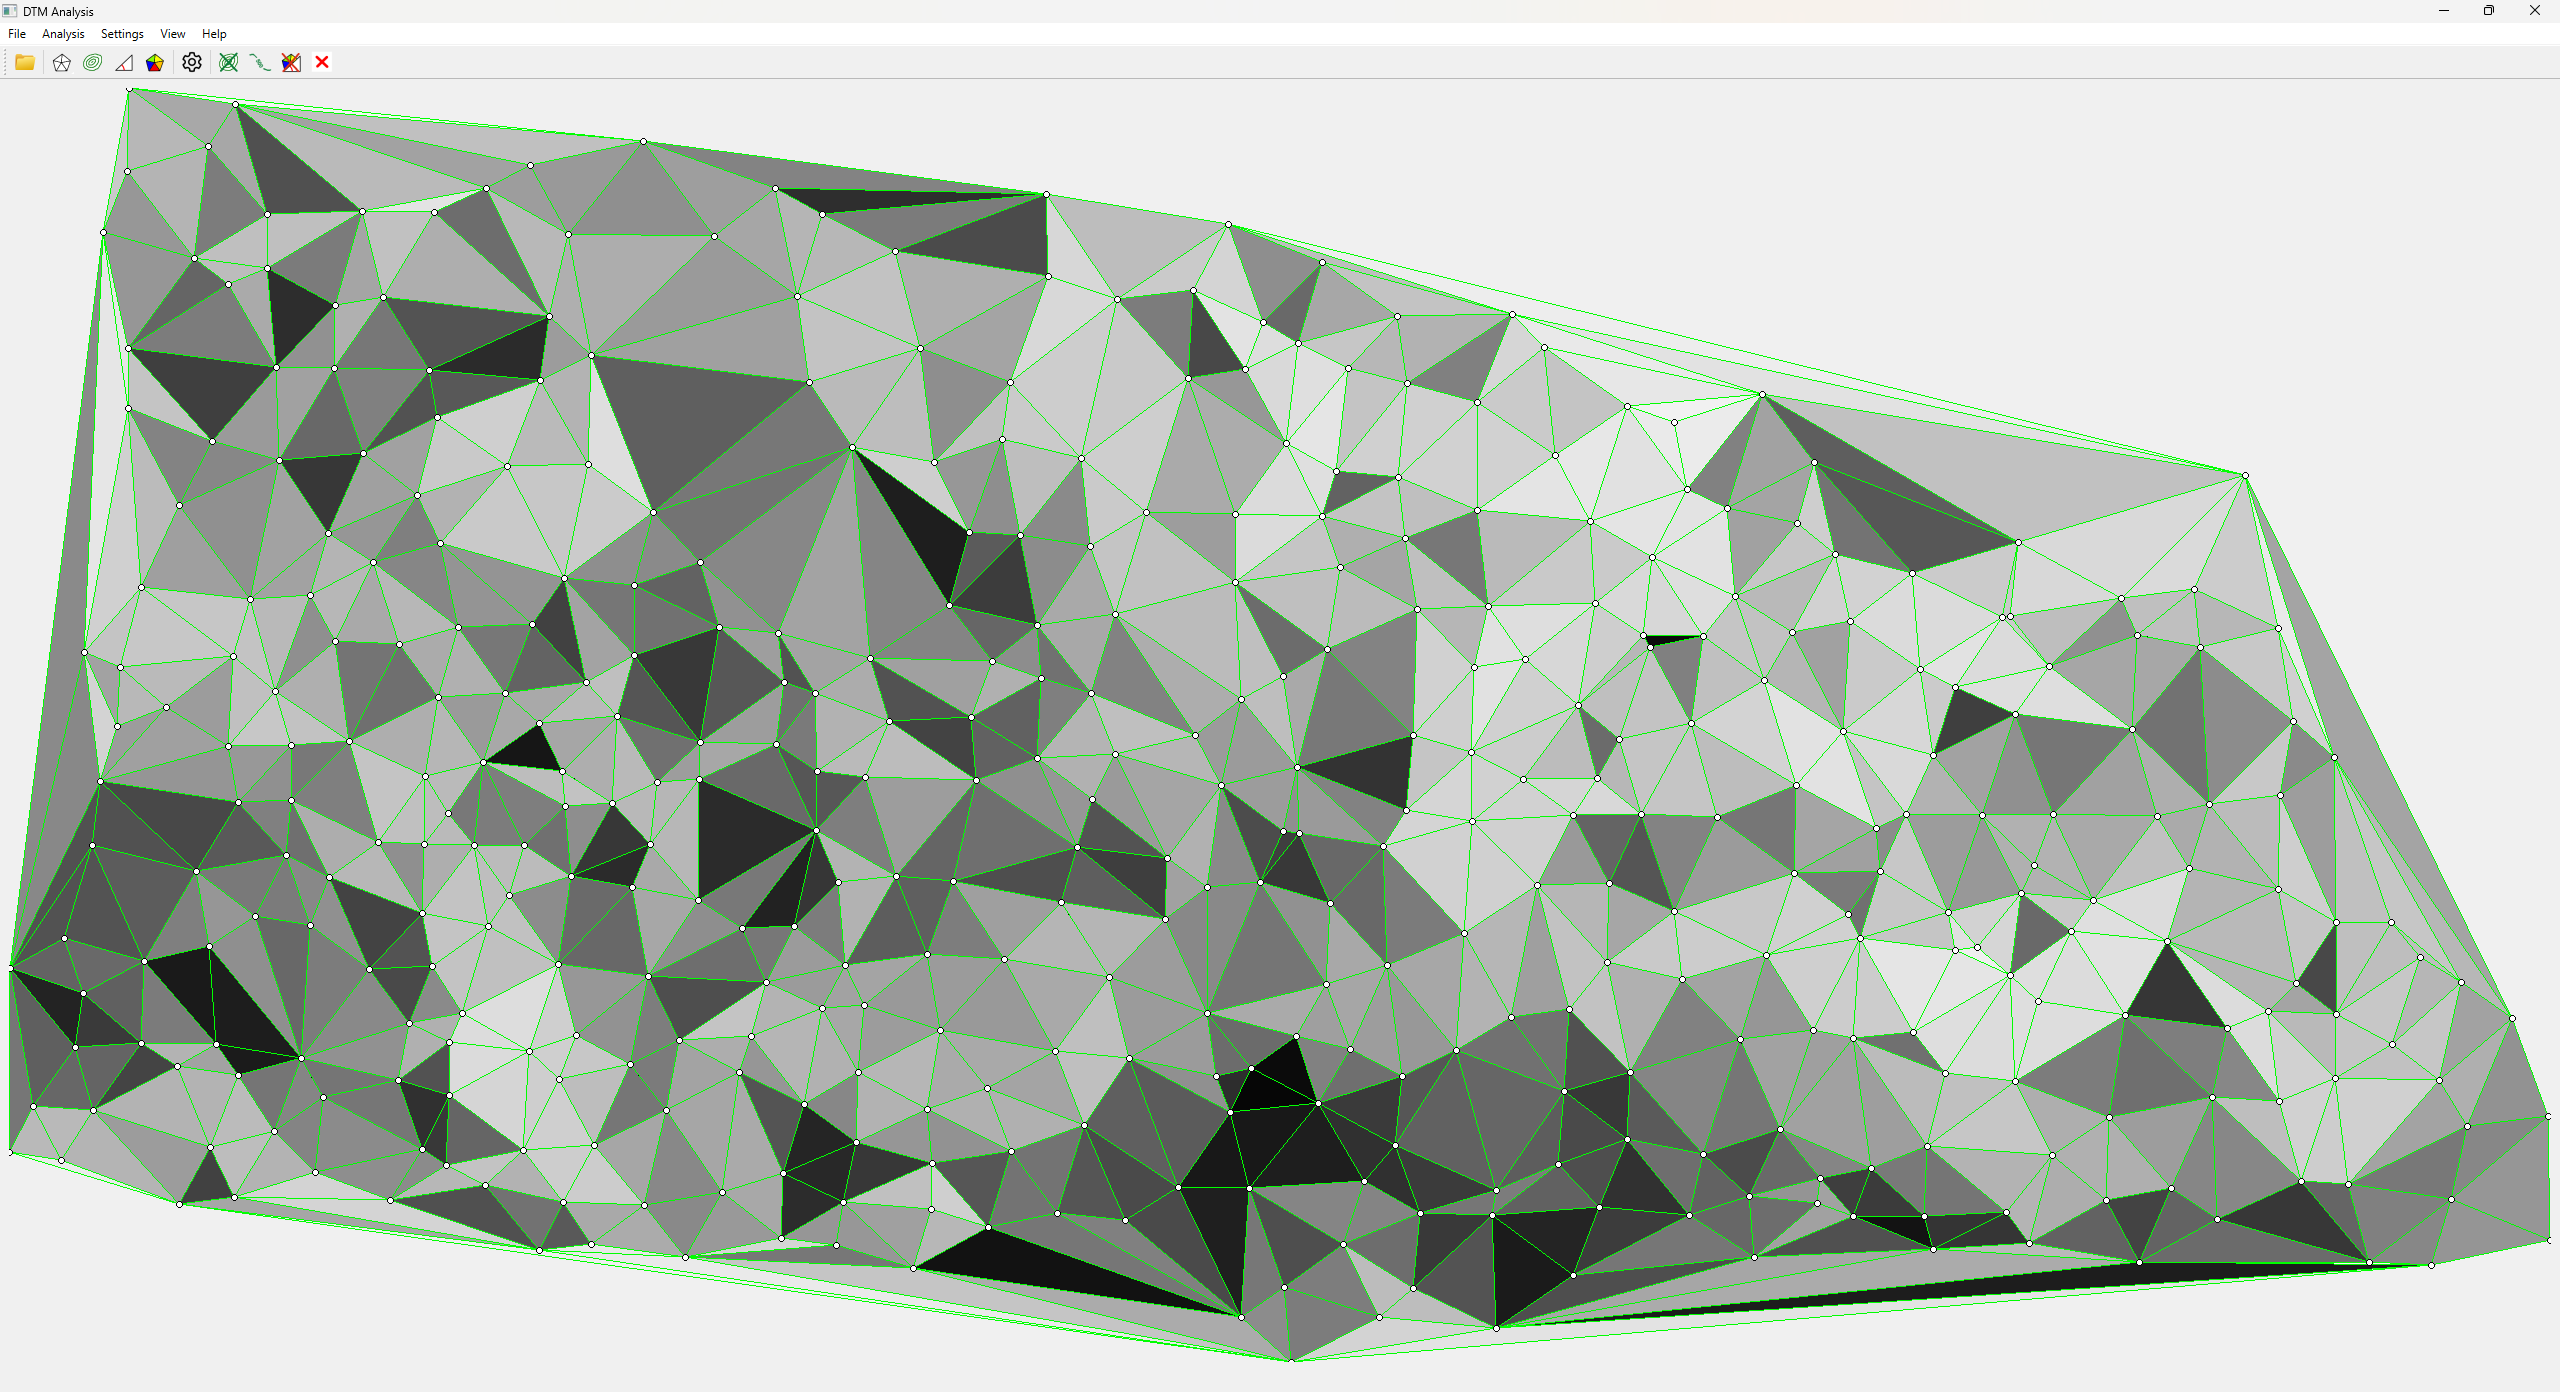
\includegraphics[width=\linewidth]{images/slopeshowcase.png}
  \caption{sklon terénu}
  \label{velcomp}
\end{subfigure}\hfill % <-- "\hfill"
\begin{subfigure}{.475\linewidth}
  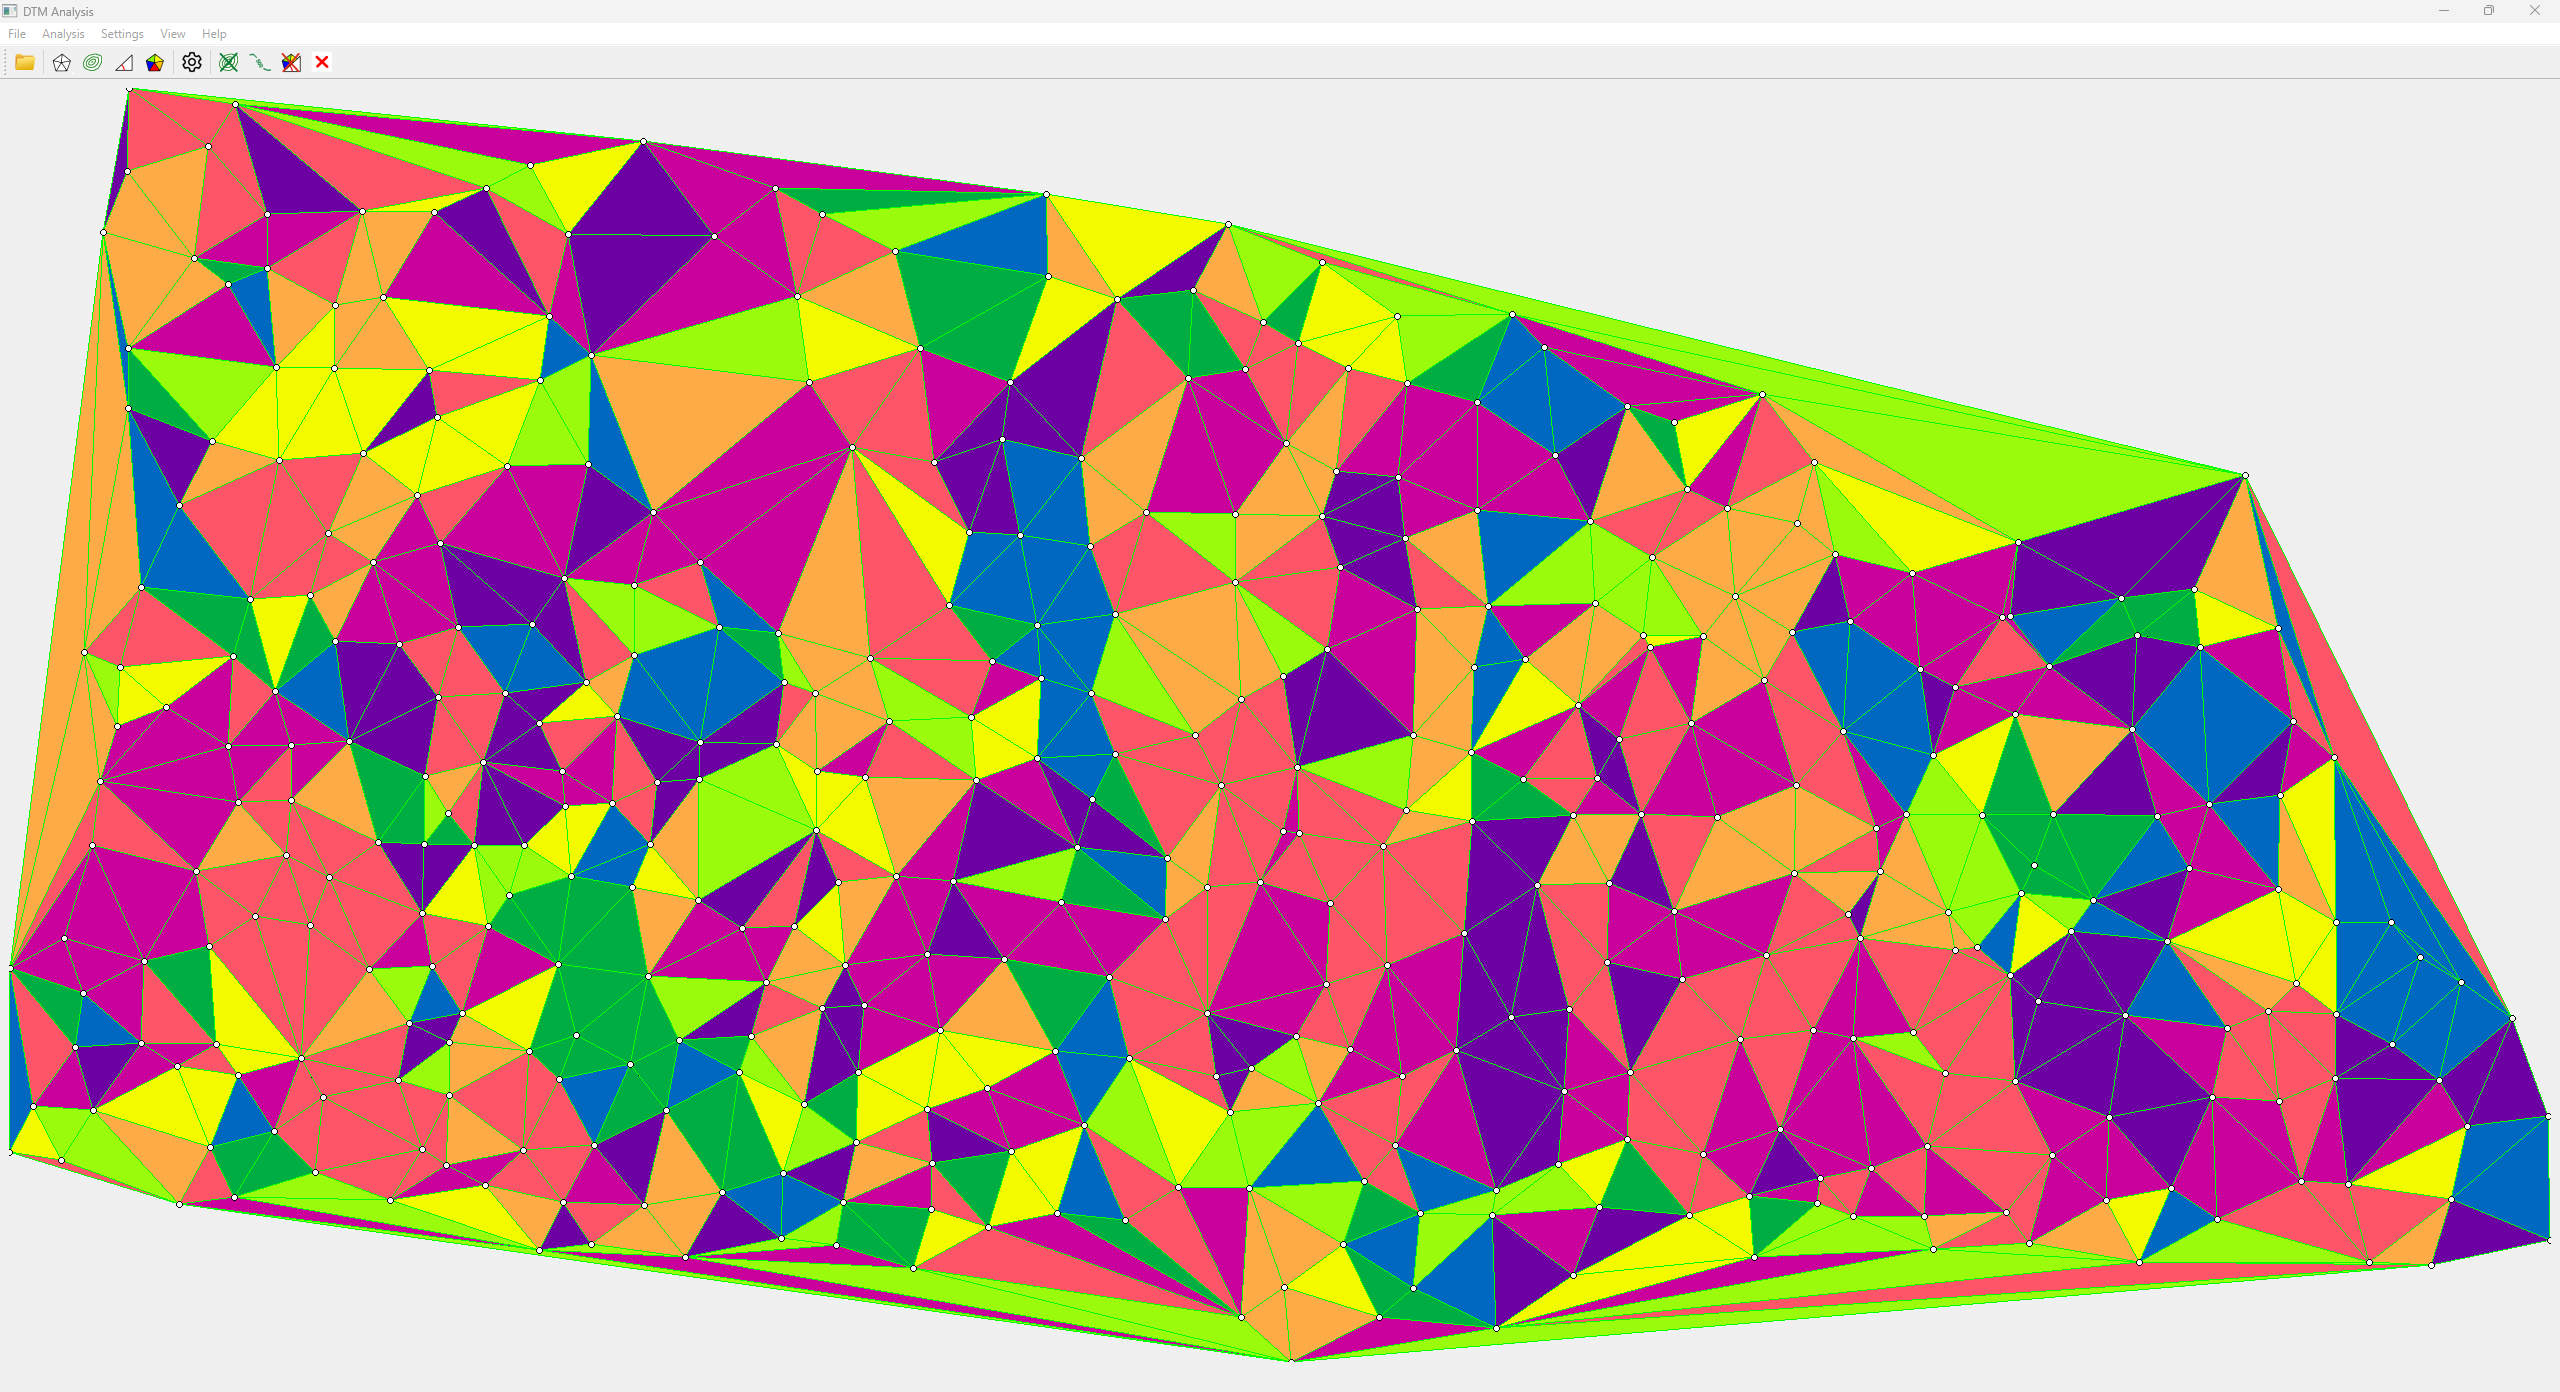
\includegraphics[width=\linewidth]{images/aspectshowcase.png}
  \caption{orientace terénu}
  \label{estcomp}
\end{subfigure}

\caption{Ukázka analytických funkcí pro DMT}
\label{fig:roc}
\end{figure}

\par Uživatel má také možnost upravit generování vrstevnic nastavením vlastního intervalu nadmořských výšek a kroku (obr. 8). Aktuální verze aplikace podporuje jen \verb|int| číselné hodnoty pro všechny nastavení. Pokud uživatel zadá nevalidní vstup nebo nevyplní všechny pole v dialogovém okně, vrstevnice se budou generovat dle výchozích nastavení přizpůsobených pro výškové poměry Česka (v intervalu 0–1\thinspace600 m n. m., krok 10 m).

\begin{figure}[H]
\centering
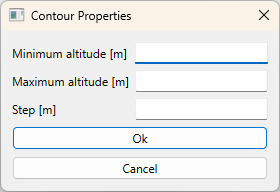
\includegraphics[width=6cm]{images/contourpropshowcase.png}
    \caption{Nastavování intervalu a kroku generování vrstevnic (vlastní zpracování).}
\end{figure}

\bigbreak

\section*{Třídy a metody}
\par Funkční chod aplikace si vyžaduje sedm povinných skriptů, v kterých jsou implementovány potřebné třídy a metody: \verb|mainform.py|, \verb|algorithms.py|, \verb|draw.py|, \verb|dialog.py|, \verb|Edge.py|, \verb|QPoint3DF.py| a \verb|triangle.py|.
\bigbreak
\par {\large\textbf{Třída MainForm} }
\par Třída MainForm ze souboru \verb|mainform.py| zabezpečuje inicializaci okna aplikace, vrchní lišty, panelu nástrojů, ikon a tlačítek. Zároveň propojuje jednotlivé interaktivní položky okna s metodami, které vykonají specifické akce. Týkají se především otevření souboru, spouštění konkrétních algoritmů apod. Část této třídy byla vygenerována v prostředí \verb|Qt Creator 9.0.1| (metody \verb|setupUi()| a \verb|translateUi()|). Níže jsou vyjmenovány nově implementované metody:

\begin{itemize}
    \item \verb|runDT()|
        \subitem{Provede výpočet DT z načteného bodového mračna.}
    \item \verb|runContourSettings()|
        \subitem{Otevře dialogové okno pro nastavení parametrů generování vrstevnic.}
    \item \verb|runContourLines()|
        \subitem{Vygeneruje vrstevnice dle nastavení.}
    %\newpage
    \item \verb|runSlope()|
        \subitem{Provede výpočet sklonu svahů nad DT.}
    \item \verb|runAspect()|
        \subitem{Provede výpočet orientace svahů nad DT.}
    \item \verb|clearButton()|
        \subitem{Zavolá metodu \verb|clearCanvas()| z třídy \verb|Draw|, která vyprázdní okno.}
    \item \verb|clearSlopeAspectClick()|
        \subitem{Zavolá metodu \verb|clearSlopeAspect()| z třídy \verb|Draw|, která smaže polygony sklonu/orientace svahů.}
    \item \verb|clearContoursClick()|
        \subitem{Zavolá metodu \verb|clearContourLines()| z třídy \verb|Draw|, která smaže vrstevnice.}
    \item \verb|showContourLabelsClick()|
        \subitem{Zavolá metodu \verb|showContourLinesLabels()| z třídy \verb|Draw|, která obstarává vykreslení popisků vrstevnic.}
    \item \verb|aboutClick()|
        \subitem{Otevře repozitář s aplikací v portálu \verb|GitHub|.}
    \item \verb|exitClick()|
        \subitem{Ukončí aplikaci.}
    \item \verb|alert(type_alert=0)|
        \subitem{Spouští upozorňovací okno podle typu upozornění definovaného indexem 0 až 3:
        \begin{itemize}
            \item[] 0 – data nenačtena
            \item[] 1 – DT neprovedena, nemožno vygenerovat vrstevnice
            \item[] 2 – DT neprovedena, nemožno vypočítat sklon terénu
            \item[] 3 – DT neprovedena, nemožno vypočítat orientaci terénu
        \end{itemize}}
    \item \verb|openFile()|
        \subitem{Otevře \verb|CSV| soubor a načte ho do proměnné.}
    \item \verb|processFile()|
        \subitem{Zabezpečuje otevření souboru. Samotný soubor načte do proměnné pomocí metody \verb|openFile()| a následně zavolá metodu \verb|clearCanvas()| pro vyprázdnění okna. Pokud je vstupní \verb|CSV| nečitelný, uživatele na to upozorní vyskakovacím oknem.}
\end{itemize}

\bigbreak

\par {\large\textbf{Třída Algorithms} }
\par V této třídě jsou obsaženy algoritmy pro konstrukci a analýzu DMT, které byly popsány v kapitole \emph{Popis a rozbor problému}. Obsahuje dvě skupiny metod:
\begin{enumerate}
    \item Metody pro samotnou konstrukci a analýzu DMT (DT, konstrukce vrstevnic, výpočet sklonu a orientace terénu);
    \item Pomocní metody pro zmíněné algoritmy (výpočet euklidovské vzdálenosti, výpočet úhlů, nalezení Delaunayovského bodu, aktualizace \emph{Active Edges List} apod).
\end{enumerate}

Algoritmy v první skupině  již byly detailně popsány výše, druhá skupina obsahuje celkem 11 algoritmů uvedených níže. Jejich podrobnější popis se nachází uvnitř této třídy ve skriptu \verb|algorithms.py|.

\begin{itemize}
    \item \verb|get2LinesAngle(p1, p2, p3, p4)|
        \subitem{Vypočte úhel mezi dvěma vstupními liniemi.}
    \item \verb|euclidDistance(p1, p2)|
        \subitem{Vypočte euklidovskou vzdálenost mezi dvěma body.}
    \item \verb|getPointAndLinePosition(p, p1, p2)|
        \subitem{Vrátí hodnotu podle polohy bodu $p$ vzhledem k linii danou body $(p1, p2)$:
        \begin{itemize}
            \item[] -1 – bod je kolineární
            \item[] 0 – bod leží na pravé polorovině
            \item[] 1 – bod leží na levé polorovině
        \end{itemize}}
    \item \verb|getDelaunayPoint(p1, p2, points)|
        \subitem{Vyhledá optimální Delaunayovský bod.}
    \item \verb|updateAEL(edge, ael)|
        \subitem{Aktualizuje seznam aktivních hran – hrany do něj přidává nebo odebírá.}
    \item \verb|getNearestPoint(p, points)|
        \subitem{Vyhledá nejbližší bod z bodového mračna k danému bodu $p$.}
    \item \verb|getContourLinePoint(p1, p2, z)|
        \subitem{Vrátí 3D bod ležící na vrstevnici.}
    \item \verb|setContourDefaultSettings()|
        \subitem{Nastaví výchozí hodnoty parametrů pro generování vrstevnic.}
    \item \verb|getNormalVector(p1, p2, p3)|
        \subitem{Vrátí normálový vektor roviny dané body $p1, p2, p3$.}
    \item \verb|createSlope(p1, p2, p3)|
        \subitem{Vypočte hodnotu sklonu roviny dané body $p1, p2, p3$.}
    \item \verb|createAspect(p1, p2, p3)|
        \subitem{Vypočte azimut určující orientaci roviny dané body $p1, p2, p3$ vůči světovým stranám.}
    
\end{itemize}
\bigbreak
\par {\large\textbf{Třída Draw} }
\par Třída Draw ze souboru \verb|draw.py| slouží pro inicializaci proměnných nesoucí prostorovou informaci, načítání a vykreslování geoprostorové informace. Tato třída má 5 \verb|list| atributů, 4 \verb|int| atributy a 1 \verb|bool| atribut pro manipulaci se vstupními daty.

\par Třída Draw pak obsahuje následující metody:
\begin{itemize}
    \item \verb|setContourSettings|
        \subitem{Zobrazí dialogové okno z třídy \verb|InputDialog| a nastaví hodnoty vstupních parametrů pro vygenerování vrstevnic.}
    \item \verb|getContourSettings|
        \subitem{Vrátí hodnoty parametrů pro vygenerování vrstevnic.}
    \item \verb|contourInvalidInput|
        \subitem{Zobrazí vyskakovací okno upozorňující uživatele na špatně zadaný vstup.}
    \item \verb|paintEvent(e)|
        \subitem{Vykresluje objekty (body a polygony) na plátno (Canvas).}
    \item \verb|getAspectColor(aspect)|
        \subitem{Vrátí barvu orientace svahu podle barevné palety z ESRI.}
        \subitem
        {
            \begin{figure}[H]
            \centering
            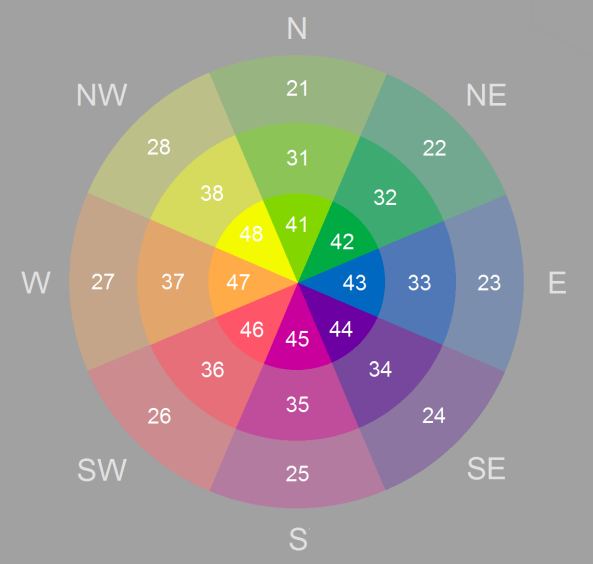
\includegraphics[width=6cm]{aspect_values.png}
                \caption{Barevná paleta expozice svahu (Buckley 2008).}
            \end{figure}
        }
    \item \verb|setDT(dt)|
        \subitem{Nastaví seznam hran v DT.}
    \item \verb|setSlopeAspect(triagles)|
        \subitem{Nastaví seznam objektů třídy \verb|Triangle| pro vykreslení polygonů sklonu/orientace terénu.}
    \item \verb|getDT()|
        \subitem{Vrátí seznam hran v DT.}
    \item \verb|getZMin()|
        \subitem{Vrátí minimální Z souřadnici.}
    \item \verb|getZMax()|
        \subitem{Vrátí maximální Z souřadnici.}
    \item \verb|getDZ()|
        \subitem{Vrátí hodnotu kroku pro vykreslení vrstevnic.}
    \item \verb|setContours(contours, index_contours)|
        \subitem{Nastaví seznam vrstevnic a seznam zvýrazněných vrstevnic.}
    \item \verb|getPoints()|
        \subitem{Vrátí bodové mračno.}
    \item \verb|switchSlopeAspect(val)|
        \subitem{Nastavuje vykreslení polygonů sklonu nebo orientace terénu na základě hodnoty $val$:
        \begin{itemize}
            \item[] -1 – nevykreslit ani sklon, ani orientaci terénu
            \item[] 0 – vykreslit sklon terénu
            \item[] 1 – vykreslit orientaci terénu
        \end{itemize}}
    \item \verb|clearCanvas()|
        \subitem{Smaže všechny objekty na plátně (Canvas).}
    \item \verb|clearContourLines()|
        \subitem{Smaže vrstevnice.}
    \item \verb|clearSlopeAspect()|
        \subitem{Smaže polygony sklonu/orientace terénu.}
    \item \verb|showContourLinesLabels()|
        \subitem{Zobrazí/skryje popisy vrstevnic.}
    \item \verb|loadData(data)|
        \subitem{Prochází vstupní \verb|CSV| soubor a načte geoprostorovou informaci.}
    \item \verb|findBoundingPoints(p,, xmin, ymin, xmax, ymax)|
        \subitem{Nalezne minimální a maximální souřadnice pro vykreslování vstupních dat.}
    \item \verb|resizeContent(xmin, ymin, xmax, ymax)|
        \subitem{Roztáhne vstupní data na plátno podle velikosti okna aplikace.}
\end{itemize}
\bigbreak
\par {\large\textbf{Třída InputDialog} }
\par Třída InputDialog dědí z předdefinované třídy \verb|QDialog| a je přizpůsobena pro zobrazení dialogového okna pro nastavení parametrů generování vrstevnic a jejich následné vracení. Obsahuje tři metody: dvě zabezpečují zpracování signálu po stisknutí příslušného tlačítka a poslední zajišťuje samotné vrácení nastavených parametrů (minimální Z souřadnice, maximální Z souřadnice, krok pro vykreslení vrstevnic). 
\bigbreak
\par {\large\textbf{Třída QPoint3DF} }
\par Třída QPoint3DF slouží pro vytvoření objektu reprezentujícího bod v 3D prostoru. Dědí atributy pro $x, y$ souřadnice z předdefinované třídy \verb|QPointF| a je jí přídělen nový atribut pro uschování Z souřadnice. Obsahuje jedinou metodu, která vrátí hodnotu Z souřadnice bodu. Všechny body vstupního bodového mračna jsou inicializovány právě jako QPoint3DF objekty.
\bigbreak
\par {\large\textbf{Třída Edge} }
\par Třída Edge slouží pro reprezentaci hrany v 3D prostoru definovanou 2 body typu \verb|QPoint3DF|. Tyto body inicializuje jako počáteční a koncový bod hrany, v rámci implementované metody je pak možné prohodit orientaci takové hrany změnou počátečního a koncového bodu – tento koncept je využit v inkrementální verzi konstrukce DT. V rámci třídy je také definovaná ekvivalentní operace pro posouzení, zda jsou dva Edge objekty shodné.
\par Pro účely určení polohy popisů vrstevnic jsou v této třídě dodatečně implementovány metody pro nalezení středu hrany promítnuté do 2D prostoru.
\bigbreak
\par {\large\textbf{Třída Triangle} }
\par Třída Triangle slouží pro vytváření objektů reprezentující trojúhelníky ve vytvořené trojúhelníkové síti. Takový trojúhelník je definován 3 body typu \verb|QPoint3DF| a navíc obsahuje atributy \verb|__slope| a \verb|__aspect| pro uložení hodnot sklonu roviny trojúhelníku nebo orientace trojúhelníku vůči světovým stranám. Třída obsahuje metody, kterými vrací konkrétní bod trojúhelníku a hodnotu sklonu/azimutu pro odečítaní orientace trojúhelníku.

